\chapter{Architecture Design}
\label{ch:Architecture Design}

\section{Technology Choices}

\subsection{Python}
We choose python as our programming language as the majority of the software written in the MANO community is in python.

\subsection{Nameko}
Nameko\footnote{\url{https://github.com/nameko/nameko}} is a micro-service framework which makes writing micro-services in python easy. It encapsulates connections, transports and concurrency making it easy for us to start implementing our application logic without the concern of underlying complexity.


\subsection{RabbitMQ}
RabbitMQ is an open source message broker software that facilitated communication between services. This is the default choice for Nameko.


\subsection{MongoDB}
MongoDB is a document-oriented database, we are using this as our persistent storage.

\subsection{Docker}
Docker is a virtualization software, which helps in easy distribution and management of applications. We are using docker to containerize our application and its dependencies.

\section{Proposed Architecture}

This section describes the architecture of SCrAMbLE (figure \ref{fig:Scramble_Architecture}). The SCrAMbLE software suite comprises of five independent micro-services (1) Translator, (2) Splitter, (3) Adaptor, (4) Gateway and (5) Main Engine.

Communication between MANO frameworks (OSM, Sonata) and SCrAMbLE is achieved through plugins which are integrated inside the MANOs, the plugins communicate through REST calls to SCrAMbLE.

The Gateway micro-service is responsible only for receiving a service request and forwarding it to the Main Engine. The Main Engine facilitates interoperability between Translator, Splitter and Adaptor micro-services, it identifies the type of service request and channels the request to the appropriate micro-service, with the help of a message broker, RabbitMQ.

All micro-services use Nameko framework to facilitate easy to use encapsulated communication between micro-services. The micro-services are all individually containerized using docker, SCrAMbLE as a whole is also containerized for easy distribution and scaling. SCrAMbLE uses MongoDB database for persistent storage.

The workflow of the individual service modules is explained in the sections below.


\begin{figure}[H]
	\centering
	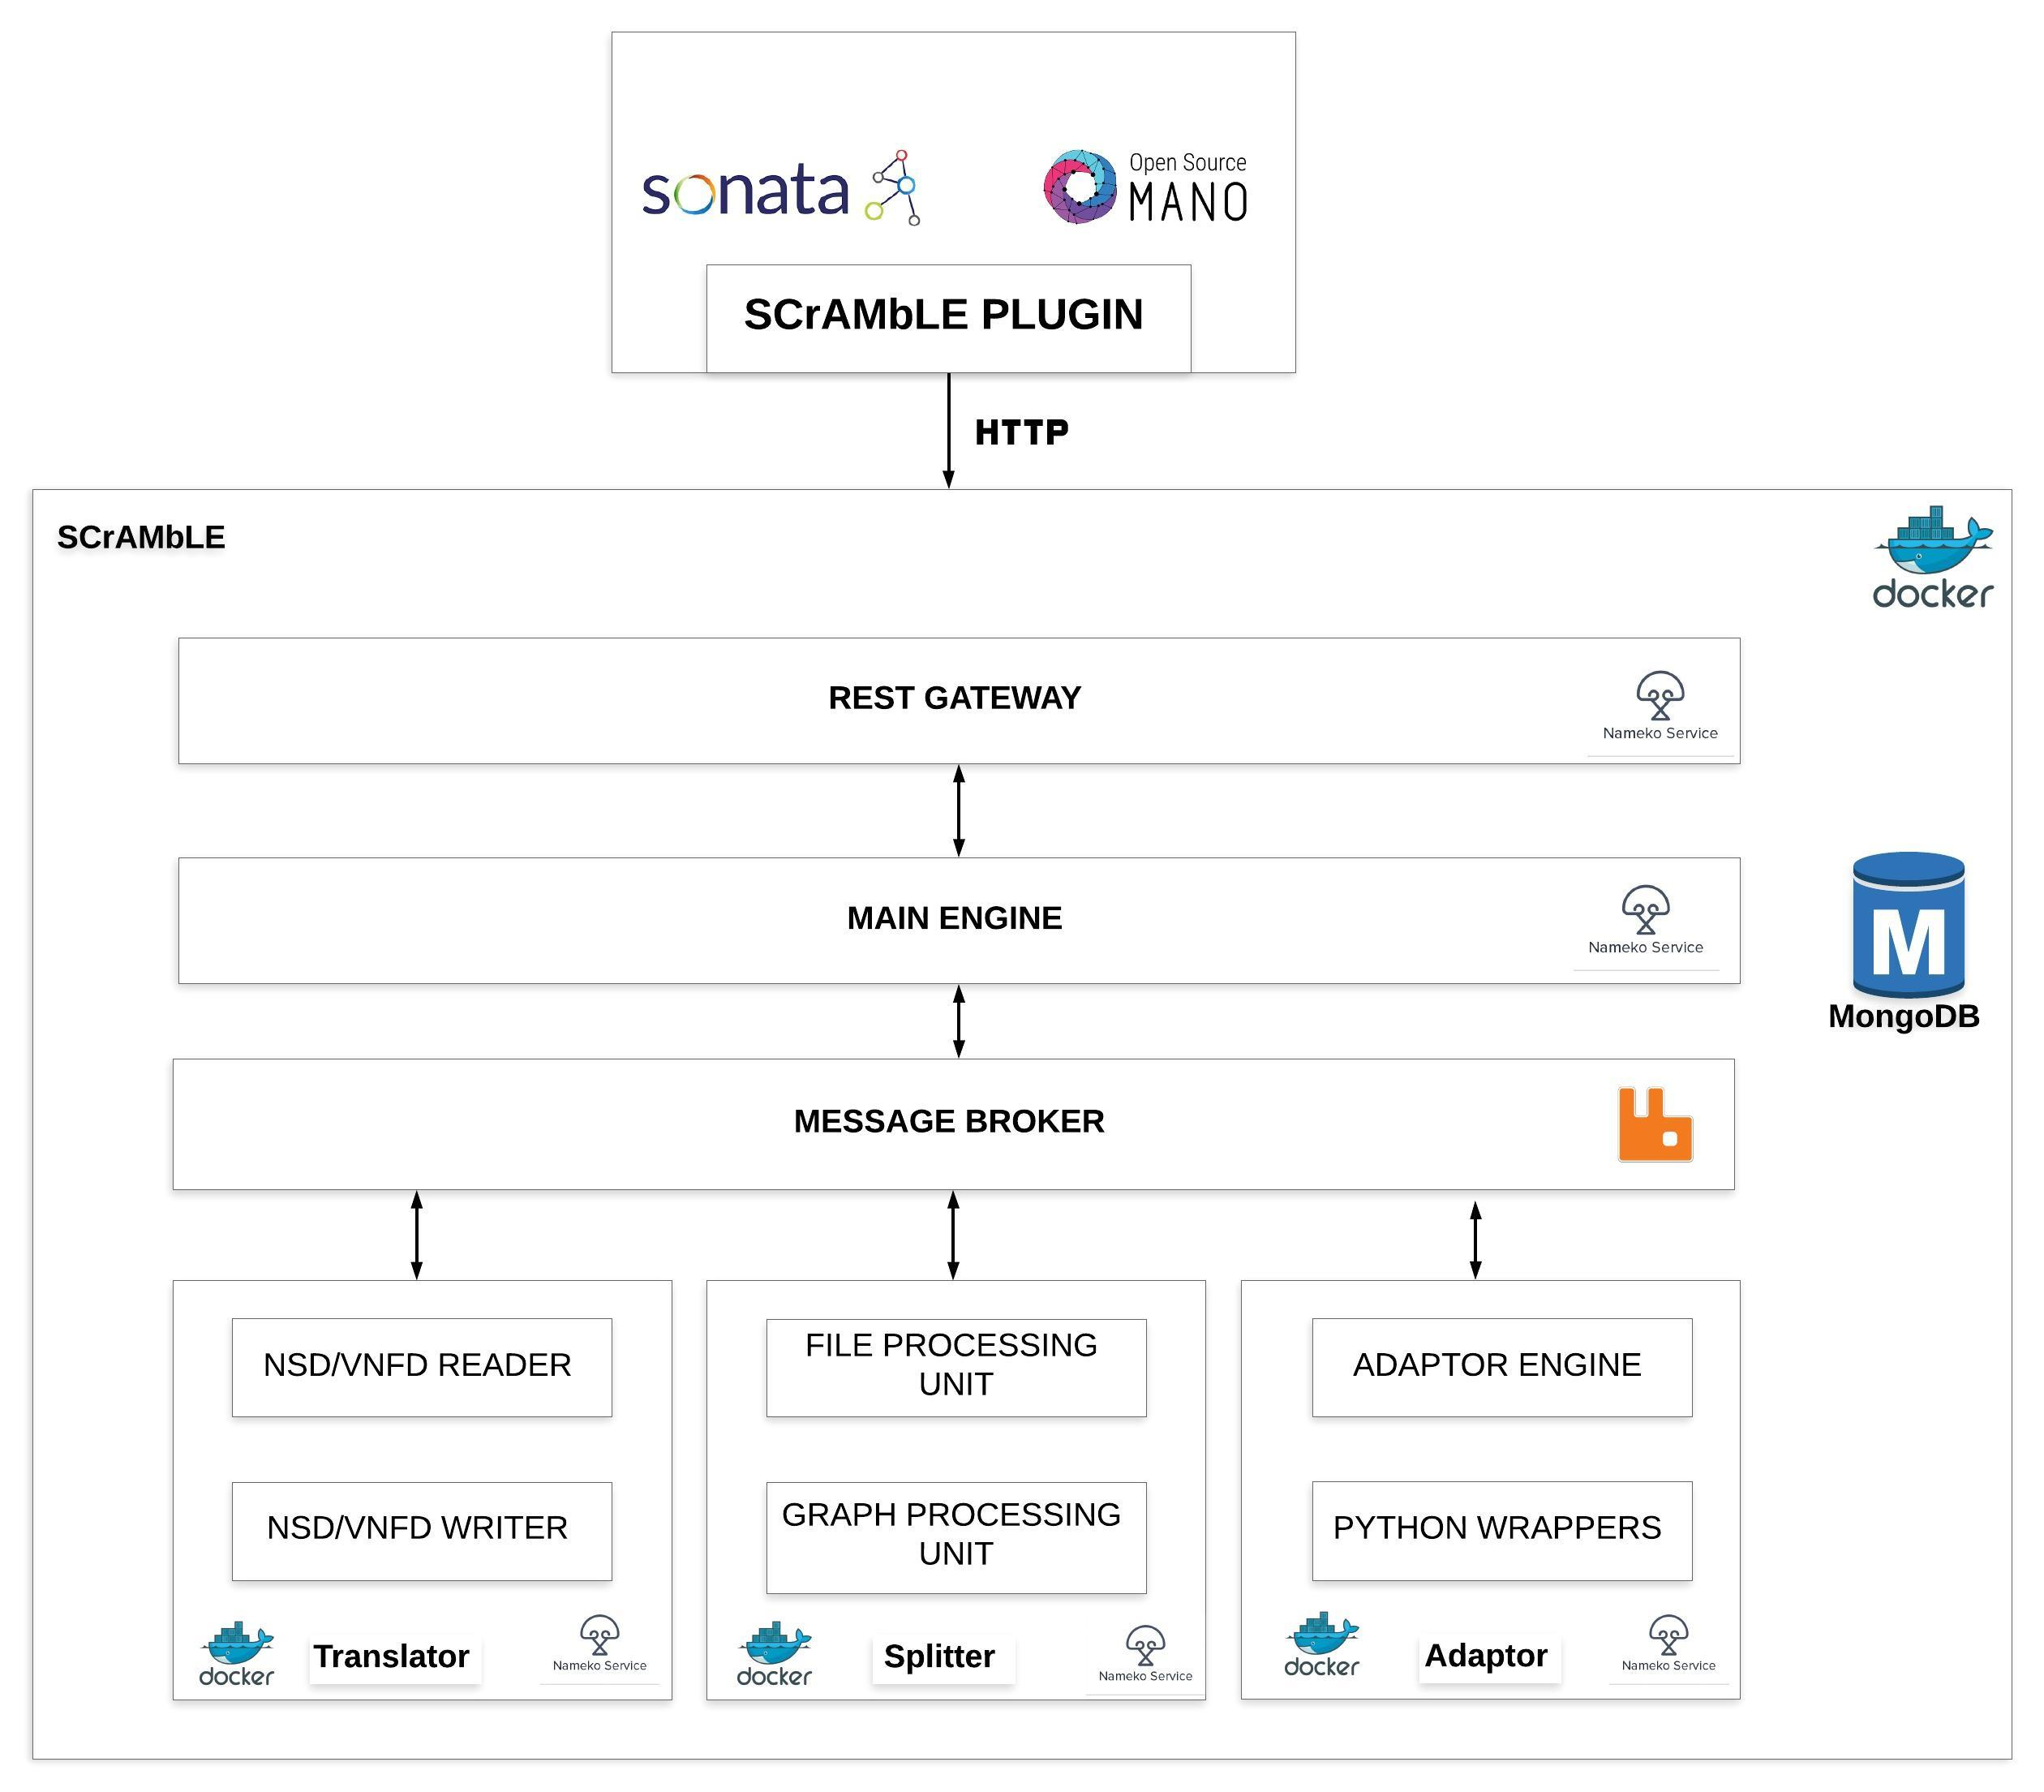
\includegraphics[width=0.9\linewidth]{figures/Scramble_Architecture}
	\caption{Project reference architecture}
	\label{fig:Scramble_Architecture}
\end{figure}

\subsection{Adaptor Workflow}
When there is a service request from any MANO to the adaptor, the request first flows to the adaptor engine (adaptor.py). Depending on the service request the adaptor engine makes a decision about the appropriate python wrapper to choose to complete the request. The adaptor engine uses the right wrapper (OSM or SONATA wrapper) to make a REST call to the target MANO. The required information is  retrieved and is finally delivered to the MANO that requests the service.
\begin{figure}
	\centering
	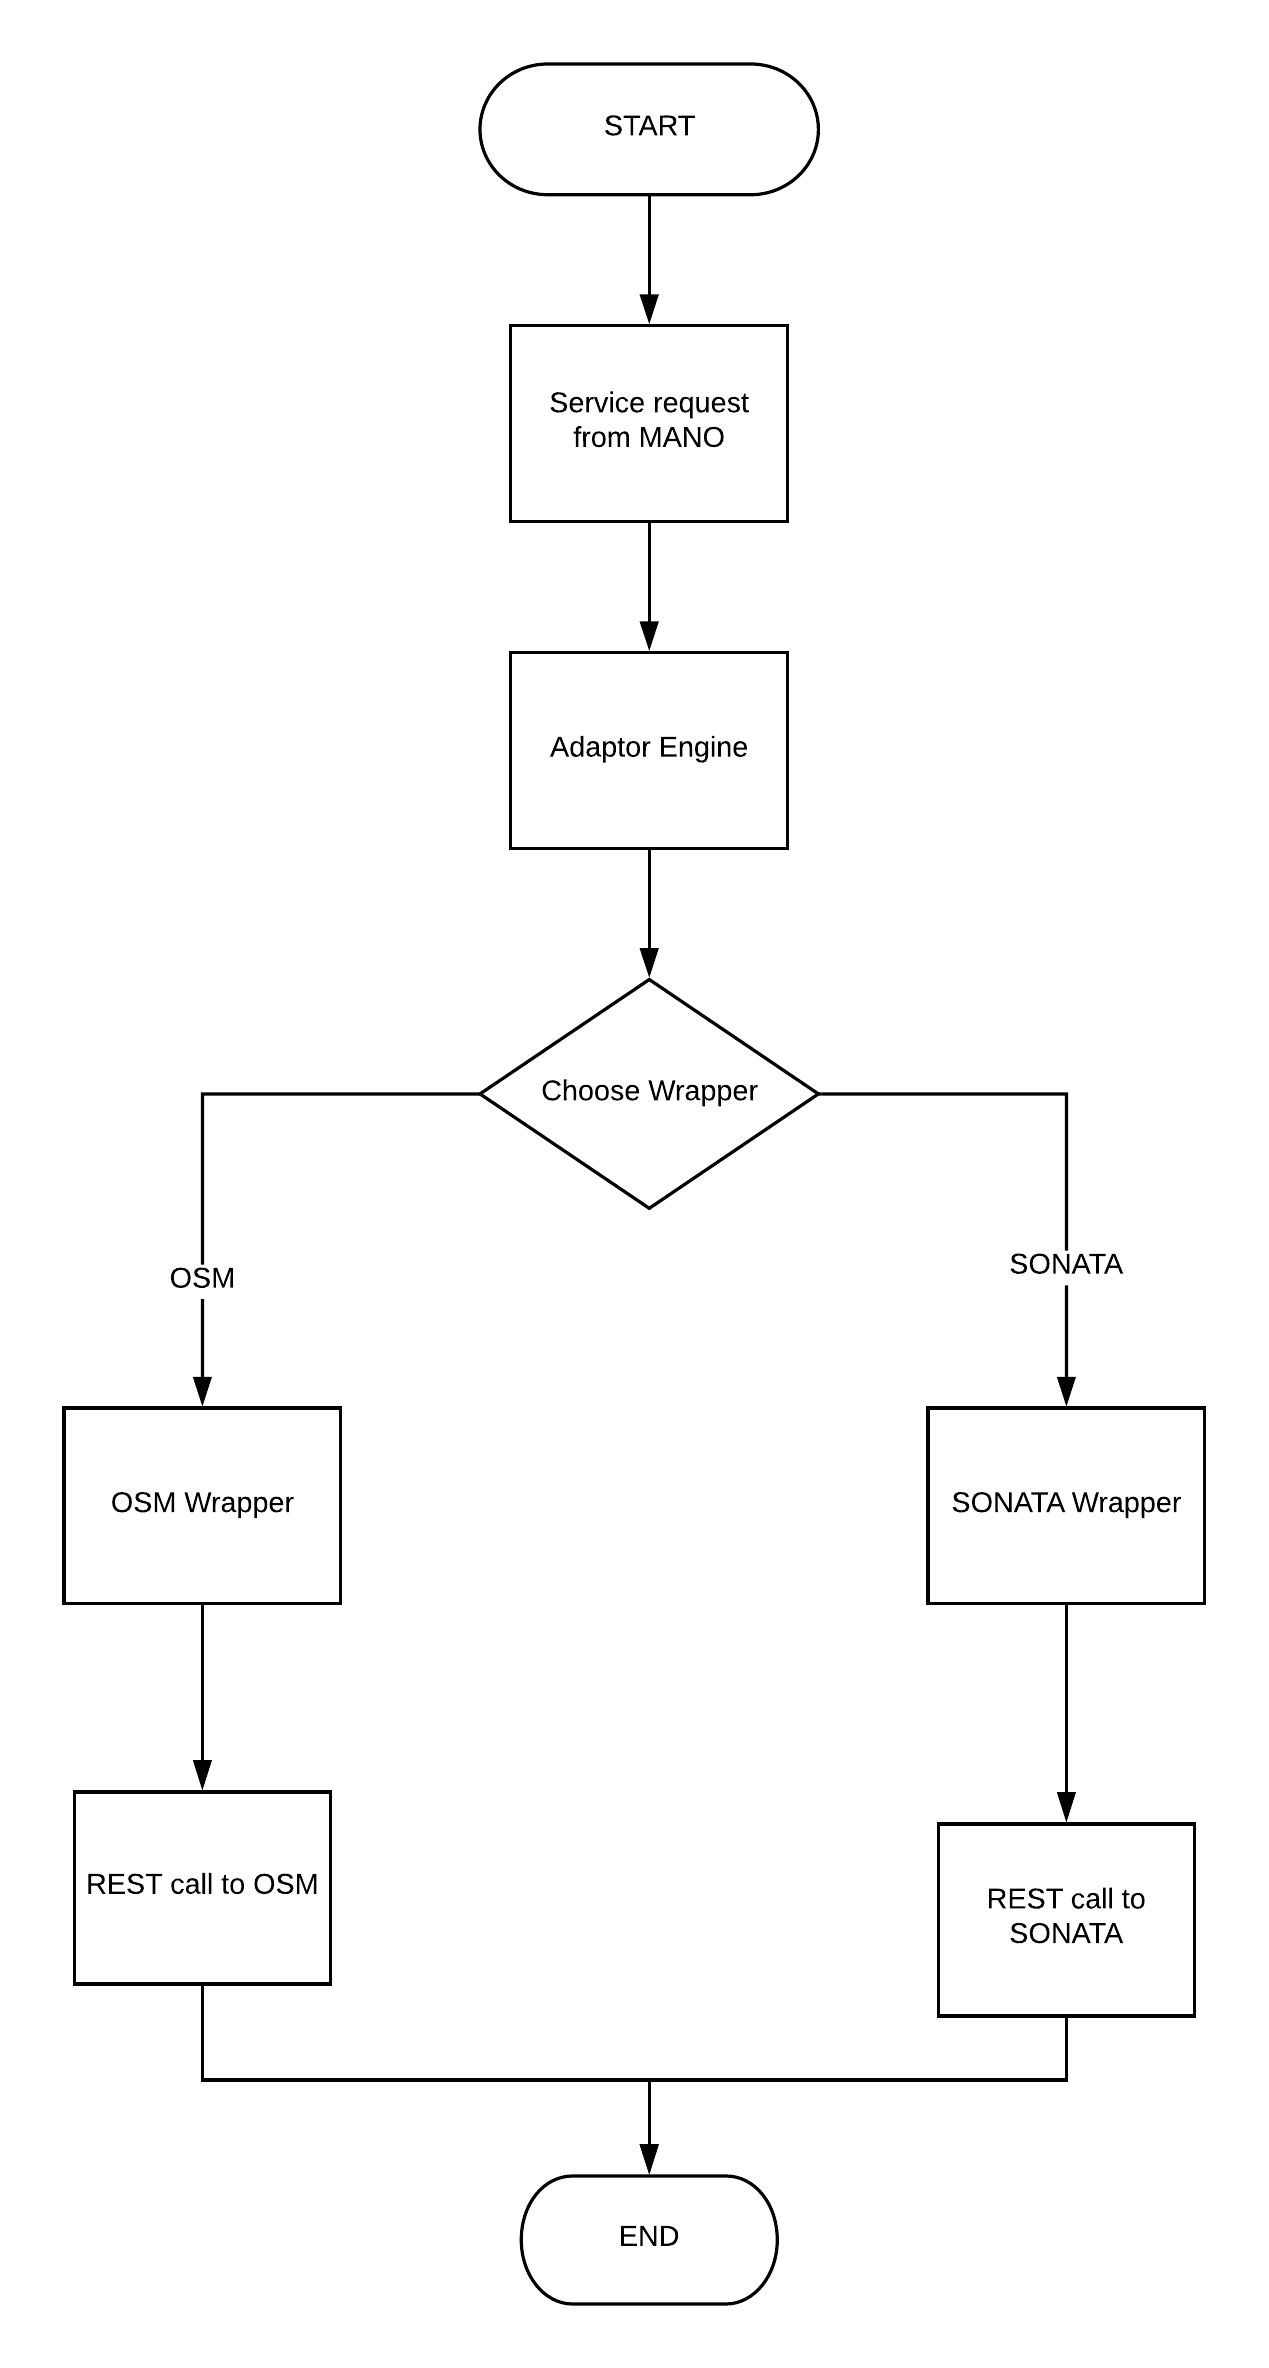
\includegraphics[width=0.7\linewidth]{figures/MA_Workflow}
	\caption{MANO Adaptor Workflow}
	\label{fig:maworkflow}
\end{figure}

\subsection{Service Descriptor Splitter Workflow}
In situations when a Network Service is to be deployed over two different MANO frameworks, splitter helps in splitting the NS into two parts. Splitter collects the reference information and fetches the NSD from the database. We will have two functional units defined, one will be file processing which basically per-processes and post-processes the file. The other functional unit is Graph splitter which actually splits the NS into two parts. Once the File processor receives the NSD file it pulls all the information related to Forwarding Graph of the NS and sends it to the graph processor. Graph processor then splits the graph into two part which results in generation of new set of nodes and sub graphs. Graph processor then forwards these two sets to file processor which creates two separate NSDs out of the two sub graphs. Splitter then either calls Translator to translate the NSDs to respective schema or it sends a reference of the two NSDs created. During the development of Splitter we might add other functional units in order to make it as modular as possible.

\begin{figure}
	\centering
	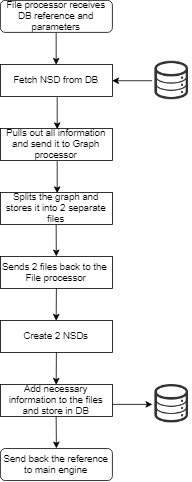
\includegraphics[width=0.5\linewidth]{figures/SDS_Workflow}
	\caption{Service Descriptor Splitter Workflow}
	\label{fig:sdsworkflow}
\end{figure}


\subsection{Service Descriptor Translator Workflow}
In a scenario where a network service is to be deployed among different MANO frameworks, having their own respective schema, SDT translates a NSD schema of one MANO framework to that of other MANO framework.
On receiving a service request to translate a NSD and/or VNFD to schema of a different MANO, the main engine stores the file(s) into the MongoDB as a document and sends a request in the form of a message to SDT usinfg Nameko services. The message contains the information of DB document name and document id, source type and destination type. 
SDT comprises of two main services, namely, a Reader and a Writer. On receiving the message from main engine, the Reader fetches the file/document from DB and validates it. After validating the file will be converted to intermediate format, which will be sent to Writer. The Writer converts the file from intermediate format to the destination file format mentioned in the request. On completion of translation, the translated file will be stored into MongoDB and the reference to the same will be passed to main engine with the service completion message.
This is an overview of the workflow for Service Descriptor Translator. The details of the message parameters communication between the components are subjected to changes in development phase.
\begin{figure}
	\centering
	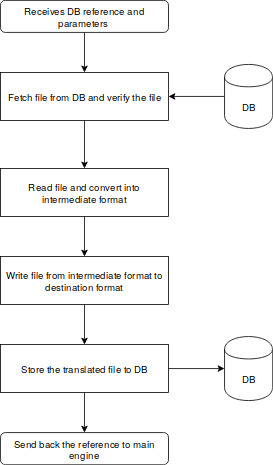
\includegraphics[width=0.5\linewidth]{figures/SDT_Workflow}
	\caption{Service Descriptor Translator Workflow}
	\label{fig:SDT Workflow}
\end{figure}

   





